% The motivation behind the development of the original fast multipole method (FMM), was the calculation of potentials in $N$-body problems,

% \begin{flalign}
%     \label{eq:ch_1:n_body}
%     \phi_j = \sum_{i=1}^N K(x_i, x_j)q_i
% \end{flalign}

% Consider electrostatics, or gravitation, where $q_i$ is a point charge or mass, and the kernels are of the form $K(x,y) = \log |x-y|$ in $\mathbb{R}^2$, or $K(x,y) = \frac{1}{4\pi|x-y|}$ in $\mathbb{R}^3$. Similar sums appear in the discretised form of boundary integral equation (BIE) formulations for elliptic partial differential equations (PDEs), which are the example that motivates our research. Consider the following integral equation formulation,

% \begin{flalign}
%     \label{eq:ch_1:generic_int_equation}
%     a(x)u(x) + b(x) \int_\Omega K(x, y)c(y)u(y)dy = f(x), \> \> x \in \Omega \subset \mathbb{R}^d
% \end{flalign}

% where the dimension $d = 2$ or $3$. The functions $a(x)$, $b(x)$ and $c(y)$ are given and linked to the parameters of a problem, $K(x,y)$ is some known kernel function and $f(x)$ is a known right hand side, $K(x,y)$ is associated with the PDE - either its Green's function, or the derivative. This is a very general formulation, and includes common problems such as the Laplace and Helmholtz equations. Upon discretisation with an appropriate method, for example the Nyström or Galerkin methods, we obtain a linear system of the form,

% \begin{flalign}
%     \label{eq:ch_1:linear_system}
%     \mathsf{K} u = f
% \end{flalign}

% The key feature of this linear system is that $\mathsf{K}$ is \textit{dense}, with non-zero off-diagonal elements. Such problems are \textit{globally data dependent} in the sense that the calculation at each matrix element of the discretised system depends on all other elements. This density made numerical methods based on boundary integral equations prohibitively expensive prior to the discovery of so called `fast algorithms', of which the FMM is an example. The naive computational complexity of storing a dense matrix, or calculating its matrix vector product is $O(N^2)$, and the complexity of finding its inverse with linear algebra techniques such as LU decomposition is $O(N^3)$, where $N$ is the number of unknowns. The critical insight behind the FMM, and other fast algorithms, is that one can compress physically distant interactions by utilising the rapid decay behaviour of the problem's kernel. A compressed `low-rank' representation can be sought in this situation, displayed in figure (\ref{fig:ch_1:low_rank}) in $\mathbb{R}^2$.

% Using the FMM the best case the matrix vector product described by (\ref{eq:ch_1:n_body}) and (\ref{eq:ch_1:linear_system}) can be computed in just $O(N)$ flops and stored with $O(N)$ memory. Fast algorithms for matrix inversion display similarly optimal scaling in the best case \cite{minden2017recursive}. Given the wide applicability of boundary integral equations to natural sciences, from acoustics \cite{wolf2011aeroacoustic,hao2015efficient} and electrostatics \cite{wang2021high} to electromagnetics \cite{darve2004fast} fluid dynamics \cite{rahimian2010petascale} and earth science \cite{chaillat2008multi}, fast algorithms can be seen to have dramatically brought within reach large scale simulations of a wide class of scientific and engineering problems. As a result the FMM has been described as one of the ten most important algorithms of the twentieth century \cite{cipra2000best}. The applications of FMMs aren't restricted to BIEs, as (\ref{eq:ch_1:n_body}) shares its form with the kernel summations often found in statistical applications, the FMM has found uses in and computational statistics \cite{ambikasaran2013large}, machine learning \cite{lee2012distributed} and Kalman filtering \cite{li2014kalman}. The uniting feature of these applications is their global data dependency.

% \begin{figure}
%     \centering
%     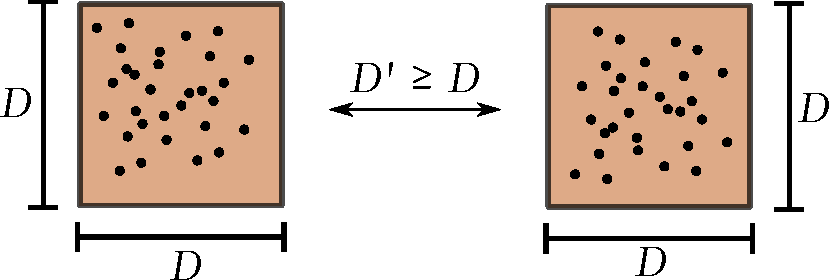
\includegraphics[width=0.7\textwidth]{ch_1/low_rank.pdf}
%     \caption{Given two boxes in $\mathbb{R}^2$, $\mathcal{B}_1$, $\mathcal{B}_2$, which enclose corresponding degrees of freedom, off diagonal blocks in the linear system matrix $\mathsf{K}_{\mathcal{B}_1\mathcal{B}_2}$ and $\mathsf{K}_{\mathcal{B}_2\mathcal{B}_1}$ are considered low-rank for the FMM when separated by a distance at least equal to their diameter, this is also known as `strong admissibility'. Figure adapted from \cite{minden2017recursive}.}
%     \label{fig:ch_1:low_rank}
% \end{figure}

% Recent decades have seen the development of numerous mathematical techniques for the computation of fast algorithms. However given their broad applicability across various fields of science and engineering, this has not been met with a commensurate development of black box open-source software solutions which are easy to use and deploy by non-experts. This is not to say that there is an absence of research software for the FMM \cite{kailasa2022pyexafmm, exafmm,wang2021exafmm,malhotra2015pvfmm, fmm3d}, or fast matrix inversion \cite{fmm3dbie, strongskel, ho2020flam}. However, the software landscape is heavily fragmented, codes often arising out of a software or mathematical investigation with infrequent maintenance or development post-publication. Few attempts have been made to re-use data structures, or application programming interfaces (APIs) between projects, and source code is often poorly documented leading to little to no interoperability between projects. Furthermore, as codes are often written in compiled languages such as Fortran \cite{fmm3d} or C++ \cite{malhotra2015pvfmm, exafmm,wang2021exafmm}, there is a relatively high software engineering barrier entry for community contributions, further discouraging widespread adoption amongst non-specialist academics and industry practitioners. Additionally, significant domain specific expertise in numerical analysis is required by users to discern the subtle differences between fast algorithm implementations, or indeed to write one independently.

% Computer hardware and architectures continue to advance concurrently with advances in numerical algorithms. Recently, the exascale benchmark (capable of $10^{18}$ flops) was achieved by Oak Ridge National Labs' Frontier machine\footnote{https://www.olcf.ornl.gov/frontier/}. With  9,472 AMD 64 core Trento nodes with a total of 606,208 compute cores, alongside 37,888 Radeon Instinct GPUs with a total of 8,335,360 cores, programming fast algorithms with their inbuilt global data dependency is challenging at a software level due to the communication bottlenecks imposed by the necessary all to all communications. Furthermore, the dense matrix operations required by fast algorithms require delicate tuning to fully take advantage of memory hierarchies on each node. Currently there exist very few open-source fast algorithm implementations that are capable of being deployed on parallel machines \cite{malhotra2015pvfmm, exafmm,}, or take advantage of a heterogenous CPU/GPU environments \cite{exafmm, h2lib2016github}. In fact for fast inverses there doesn't yet exist an open-source shared memory implementation. Furthermore, developers must using existing codes must employ careful consideration in order to successfully compile the software in each new hardware environment they encounter, from desktop workstations to supercomputing clusters.

% Resultantly, researchers who may want to write application code that takes advantage of fast algorithms as a black box without the necessary software or numerical analysis expertise to implement their own have few choices, and fewer still in a distributed computing setting. Identifying this as a significant barrier to entry for the adoption of fast algorithms in the wider community, we propose a new unified framework for fast algorithms, beginning with an implementation of a parallel FMM, which we introduce in the following section, designed for modern large scale supercomputing clusters. We emphasise our focus on ergonomic and malleable code, such that our code is easy to edit and deploy on a multitude of architectures while still achieving good scaling. With a key target application being the simulation of exascale boundary integral problems for electromagnetics, specified by Maxwell's equations.

Q. What are the constraints of scientific software development, in an academic setting?
    - Small team
    - Require cross platform, performance, rapidly extensible to try out new things.

Q. What do we therefore ideally want from a programming environment?
    - trivial cross platform builds
    - easy, bug free, and performant multithreading
    - simple syntax that prioritises readability and simple code organisation, over dogmatic software design principles such as object oriented programming, that can even sacrifice performance.
    - can write C++/C extensions, to connect to other languages.
    - simple, good compiler.

Q. Why did Python and Numba not work out?

    - Long compilation times as JIT runtime-compiled.
    - Difficult to anticipate behaviour of compiler as a programmer.
    - Programming for performance was not as trivial as
    advertised for a complex algorithm, FMM.
    - just as hard as writing in compiled language, with the added barrier of having to understand how and why numba was doing certain things. Easier just to work in compiled language, and the two language problem remains.

Q. Which compiled language did you choose and why?
    - C++ has come a long way, however has many pitfalls.
        - complex build system, and diverse set of compilers.
        - smart pointers are great.
        - complex, overlapping, syntactic features. Too many ways of writing the same thing. There's some dicussion about this in old upgrade.

    - Rust is fresh, designed for performance like C++, but without historical baggage.
        - syntax is clear, functional when it needs to be, and oop when it needs to be. Traits emphasise the behaviour expected from a piece of code in contrast to inheritance.
        - outstanding cross platform builds, based on LLVM so should in theory have no performance differences from modern C++ or Fortran.
        - Easy to write to C ABI, and make Python interfaces, or interfaces to existing C/C++ libraries.
        - Unified build, test, doc in the runtime.


Q. What else is out there?
    - Python has emerged as a defacto standard for data science, and machine learning, which are numerically intensive. New projects, such as Python 3.12, - removes GIL
        - MOJO language.

    - Are perhaps the future, but Mojo is still in its infancy, and is not open source, it's too early to say, and for now Rust+Python offers a great programming environment for scientific software development.

    - Julia is a JIT compiled language too, and is prey to the same pitfalls as Python/Numba for performance its hard to manually manage memory, and its imperfect. There are other pitfalls in Julia, like distributed memory programming, and build times in distributed memory programs.


% - The goal of this research project is to contribute significantly towards the design and development of a highly-parallelised, scalable, software infrastructure for `Fast Algorithms'
%     - `Fast Algorithms' - explain how they arise from desnse matrices with hierarchical structures that allows for numerical compression of off-diagonals for optimal application/inversion.
%     - Specific outputs:
%         - Parallel tree library
%         - Parallel FMM library
%         - Re-use of data structures to create fast direct solver library.
%     - Context
%         - Next gen BEM software
%             - can scale from laptops to supercomputers
%             - deployed with ease with interpreted language interfaces for non-computational researchers
%         - Problems that can be studied
%             - virus simulation
%             - geophysics
%             - ML
%     - Impact
%         - solvers in this domain are either
%             - designed to numerically validate an algorithmic approach
%             - heavily optimised to achieve performance
%         - nothing extensible really available
%             - as a testbed for algorithmic experimentation
%             - extension to differing applications in which these algorithms apply.
%             - or as a testbed for new implementation approaches
%                 - new hardware etc.
%         - the impact of a particular method is defined by how easy it is for software to be extended OR to be run as a black box.
